% Chapter 2

\chapter{Fundamentação Teórica}\label{chap:background}


\section{Área dos Negócios}\label{sec:business}


\section{Fundamentos da Área}\label{sec:fundamental}

Equação ~\ref{eq:my_equation} é um exemplo de uma equação em Latex:


\begin{equation}\label{eq:my_equation}
    h_t = f(W^{(hh)}h_{t-1} + W^{(hx)}x_t).
\end{equation}


Figura\ref{fig:diagram} é um exemplo para incluir uma figura.

\begin{figure}[htb]
    \caption{Simple diagram}
    \centering
    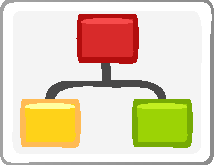
\includegraphics[scale=1.9]{img/diagram.pdf}
    \label{fig:diagram}
    \source{Retirado de \cite{larcc}.}
\end{figure}

\cite{GRIEBLER:IJPP:18}


\cite{MACCOOL:structured_patterns:book:12}


\section{Trabalhos Relacionados}\label{sec:rw}

São apresentados neste tópico, os trabalhos relacionados, que possuem
algum ponto em comum com o que se quer realizar no presente projeto.
Pretendesse aqui, identificar estes pontos, e compará-los com a proposta deste projeto.

\subsection{BDTC - Uma Biblioteca Digital de Trabalhos Científicos com Serviços Integrados}

O trabalho desenvolvido por \cite{CERVI:bdtc}, possui como premissa a apresentação
de uma proposta de biblioteca digital de trabalhos científicos, que foi denominada como
BDTC, que possui como objetivo prover o suporte a três pontos fundamentais:
auto-arquivamento do conteúdo, extração de metadados e busca de similaridade.

Como um dos principais diferenciais, foi desenvolvido um mecanismo de
busca por similaridade para as pesquisas realizadas na BDTC,
que permite ao usuário encontrar trabalhos relacionados, mesmo que
parte da palavra pesquisada não seja exatamente igual ao conteúdo presente
no documento.

Para o desenvolvimento deste mecanismo de busca, foi utilizado
um recurso denominado \emph{n-gram}, que permite quebrar uma palavra em
conjuntos de letras de tamanhos variados, é retratado como exemplo o
\emph{3-gram} do termo "Juci", que pode ser quebrado em dois conjuntos de 3
letras, ou seja, \emph{"Juc"} e \emph{"uci"}.

Estes conjuntos são armazenados em uma tabela de indices no banco de
dados, de forma que ao realizar uma consulta a partir de uma palavra,
o sistema retorna todos os trabalhos que contenham algum dos conjuntos
de letras que compõem a palavra pesquisada.

Em relação com o presente projeto, pode ser realizado uma comparação com
a forma como o mecanismo de busca foi desenvolvido na BDTC. Ao envés de
utilizar o recurso de \emph{n-gram}, o sistema proposto neste projeto utilizara
o recurso de \emph{tokenization} presente na ferramenta de Full Text Search do
banco de dados PostgreSQL, que possui um resultado final semelhante, porem não
idêntico, visto que o \emph{tokenization} remove o gênero das palavras,
os espaços em branco, palavras comuns e palavras que não são consideradas relevantes.

\subsection{Desenvolvimento da nova Biblioteca Digital da Biblioteca Brasiliana USP: Relato de Experiência}

O relato de experiência desenvolvido por \cite{GarciaRodrigoMoreira2019DdnB}
apresenta o desenvolvimento da na nova plataforma de Biblioteca Digital da
BBM, a Biblioteca Brasiliana Guita e José Mindlin, em forma de retrospectiva
desde o projeto-piloto, relatando os principais problemas, êxitos
e desafios encontrados durante o desenvolvimento do projeto, que envolvia
a digitalização e desenvolvimento de uma coleção digital para a biblioteca.

A Biblioteca Brasiliana Guita e José Mindlin foi inaugurada em março
de 2013, sendo um órgão e entidade acadêmica da Pró-Reitoria de Cultura
e Extensão da USP (Universidade de São Paulo). Este biblioteca envolve o
projeto Brasiliana USP, que foi iniciado em 2005, e tem como objetivo
abrigar a coleção Brasiliana, doada por José Mindlin. Dentro do escopo
deste projeto, em 2008 é iniciado o projeto-piloto da Biblioteca
Brasiliana Digital, que visa a preservação do acervo e democratização
do acesso ao material.

Para o desenvolvimento da biblioteca digital, foi optado por realizar uma
customização do sistema DSpace, um software open source de repositório
digital, com recursos como o Djatoka (servidor de imagens) e visualizadores
de livros como IIPImage e BookReader.

Como principais problemas e êxitos, foi ressaltado a forma como as customizações
foram realizadas no DSpace, sendo muitas delas realizadas diretamente no código fonte
do programa, tornando extramente difícil ou até impossibilitando a atualização
para novas versões da plataforma. Resultado em inconsistências na
visualização dos documentos digitalizados, lentidão do sistema, dentro outros
problemas que vieram a surgir ao longo do tempo.

Além disto, também foi relatado a rotativada das equipes como um fator de impacto
para a continuidade do desenvolvimento da biblioteca, que em sua
maioria era constituída por bolsistas, estagiários e poucos profissionais
terceirizados contratados por tempo determinado. Também foi constatado
que as máquinas digitalizadoras adquiridas para a biblioteca não eram
adequadas para o manuseio dos documentos do acervo, visto que os documentos
eram obras raras, e que necessitavam de diversos cuidados para a preservação
e conversação do material.

Com o tempo parte dos problemas foram resolvidos, sendo até adquirido novas
maquinas digitalizadoras, mais modernas e adequadas para o manuseio do material
bibliográfico.

Comparando o trabalho relacionado com o presente projeto de pesquisa,
é possível ressaltar que o atual projeto não tem como intenção a digitalização
de um acervo físico, porem o sistema DSpace que foi utilizado no trabalho
relacionado foi identificado como um sistema muito popular para o desenvolvimento
de repositórios acadêmicos e bibliotecas digitais de universidades, sendo
possível utilizar a experiência adquirida na implantação desse sistema durante
o desenvolvimento do repositório acadêmico proposto.

\subsection{Classificação facetada: proposta de categorias fundamentais para organizar teses e dissertações em uma biblioteca digital}

O artigo desenvolvido por \cite{PereiraClaytonMartins2021Cfpd} tem como
proposta a apresentação de categorias fundamentais, baseadas nos trabalhos
do matemático e bibliotecário indiano S. R. Ranganathan e do \emph{Classification Research Group}, que pode ser utilizadas
durante o desenvolvimento de interfaces de navegação facetada de bibliotecas
digitais e repositórios de dissertações e testes.

Neste trabalho é relatado que é comum em bibliotecas digitais de teses
e dissertações, encontrar problemas referente a facilidade de encontrar
e recuperar documentos neles armazenados, visto que a principal forma de
pesquisa tende a ser por um campo textual, onde é possível efetuar buscas
simples, e em alguns casos utilizar a combinação de operadores lógicos, como
\emph{AND}, \emph{OR} e \emph{NOT}, para buscas mais complexas.

Porem esta forma de pesquisa, por meio de um único campo textual,
exige que o usuário possua conhecimento prévio de noções de logica,
sigla dos cursos, areas e linhas de pesquisa, e que seja capaz de
utilizar essas informações para construir uma busca mais complexa,
geralmente fazendo com que as pesquisas realizadas retornem resultados
vazios, ou não exibam o total potencial de documentos contidos na plataforma,
levando em consideração questões semânticas dos termos utilizados na pequisa.

Desta forma, a abordagem de pequisa facetada permite que o usuário navegue
pela estrutura conceitual das informações armazenadas no repositório, além de
combinar conceitos de diferentes perspectivas ou facetas (janelas ou menus), sendo uma abordagem
de pesquisa mais eficiente, auxiliando o usuário a encontrar o que procura,
de forma visual e intuitiva a partir de palavras chaves modificáveis em um
vocabulário controlado.

Como resultado de sua pesquisa, foram obtidos as seguintes categorias
fundamentais, seguidas de um exemplo: Documento (Trabalho de conclusão), Tipo (Dissertação, Tese);
Curso (Meteorologia); Linha de Pequisa (Sensoriamento);
Tema (Anomalias climáticas); Especialização do tema (Conservação de Energia);
Localização (Oceano Atlântico); e Ano de publicação (2020).

Em relação ao atual projeto de pesquisa, as categorias fundamentais encontradas
no trabalho relacionado poderiam ser utilizadas para a organização dos documentos dentro do repositório
de trabalhos acadêmicos proposto, podendo ser utilizados em recursos de
filtragem das publicações dentro da plataforma.

\subsection{Garantindo acervos para o futuro: Plano de preservação digital para o Repositório Institucional Arca}

A pesquisa realizada por \cite{QueirozArca:2020} tem como objetivo
apresentar o desenvolvimento do plano de ação de preservação digital
para o Arca - Repositório Institucional da Fiocruz, visando descrever
as ações necessárias para garantir a preservação dos documentos, bem como
a adoção de padrões, procedimentos e tecnologias que possam ajudar a garantir
a preservação do seu acervo digital para o futuro.

O repositório institucional da Fundação Oswaldo Cruz (Fiocruz) denominado
Arca, foi criado em 2007 e lançado oficialmente como repositório institucional em 2011,
utilizando como o base o \emph{software open source} Dspace, e tendo como intuito
reunir, hospedar, disponibilizar e dar visibilidade a produção intelectual e cultural
produzida na fundação.

Como padrão referência, o artigo cita o \emph{Open Archival Information System}
(OAIS), presente na norma ISO 14721:2003, e adaptado na normal brasileira
NBR 15472:2007. O OAIS define um modelo para configuração e operação
de um repositório digital de documentos confiável, descrevendo como deve funcionar
a estrutura e fluxo das informações, desde a inserção dos documentos digitais e
metadados, até a forma como ocorre o seu armazenamento e acesso.

Dentre as repensabilidades obrigatórias para atender o modelo OAIS
está a documentação das políticas e procedimentos para garantir
a preservação dos documentos a longo prazo, bem como o plano de ação
de sucessão caso o repositório seja desativado ou substituído por outro.

Como resultado de sua pesquisa, foi elaborado uma estrutura básica
do Plano de Ação de Preservação Digital, onde em primeiro momento
é descrito os elementos essenciais para a preservação, como: o cenário
institucional, a descrição da coleção, avaliação de riscos e ameaças,
e o planejamento das estrategias para prevenção de obsolescência. E em
segundo momento, é optado por uma combinação de estrategias de preservação
a serem aplicadas, como a normalização de formatos de arquivos, e a verificação
periódica do formato dos arquivos em uso, que possam apresentar riscos
de obsolescência tecnológica.

Como contribuição ao atual projeto de pesquisa, pode ser citado a
apresentação ao padrão OAIS, que pode ser utilizado durante o desenvolvimento
do repositório acadêmico, visando a conformidade com padrões internacionais
de desenvolvimento de repositórios acadêmicos confiáveis, além da apresentação
de um plano de ação de preservação digital, que envolve a sucessão das obras
armazenadas em caso de desativação ou substituição do serviço.

\subsection{O mapeamento dos repositórios institucionais brasileiros: perfil e desafios}

O artigo realizado por \cite{Weitzel:2019} tem como objetivo mapear
os repositórios institucionais brasileiros até o período de maio de 2017,
com a finalidade de identificar a atual situação de conformidade com
a estrategia do Acesso Verde Aberto proposto pela BOIA (\emph{Budapest Open Access Initiative}),
além de contribuir com a orientação de diretrizes nacionais e internacionais
para implementação e desenvolvimento de repositórios institucionais, ou sua integração
em rede.

A BOIA (\emph{Budapest Open Access Initiative}) estabelece duas estratégias
de Acesso Aberto, sendo a primeira o Acesso Aberto Dourado, que se baseia
nos esforços da comunidade cientifica para criar um ambiente ideal onde
os periódicos eletrônicos são disponibilizados sem cobrança de assinaturas
ou taxas impostas pelas editoras, como as APCs (\emph{Article Processing Charges}).
A segunda estratégia é o Acesso Aberto Verde, onde o próprio autor
realiza a publicação de seu periódico, seja a versão inicial ou
final, em um repositório institucional.

Para a realização do estudo, foi realizado um levantamento de dados em
fontes como o OpenDOAR, ROARMAP, ROAR, Lista de Repositórios do IBICT,
edital da FINEP, lista de usuários do DSpace e os repositórios listados
no \emph{The Ranking Web of World Repositories}. Como indicador de
alinhamento com o Acesso Aberto Verde, foi realizada a observação
direta sobre cada um dos repositórios, de forma a verificar se o mesmo
disponibiliza o acesso aos artigos de periódicos.

Como resultado, foi constatado que cerca de 54,5\% dos 101 repositórios
analisados estão alinhados com o Acesso Aberto Verde, concentrando 97,5\%
do total de artigos disponíveis em repositórios brasileiros. Também foi
identificado que os sites agregadores de repositórios mundiais não
expressam a realidade, contendo informações mal catalogadas,
\emph{links} quebrados, dentre outros problemas.

Em relação ao atual projeto de pesquisa, é possível citar a contribuição
por meio da apresentação dos conceitos de Acesso Verde Aberto e Acesso
Dourado, que visam disponibilizar os artigos de periódicos em repositórios
institucionais, sem cobrança de taxas ou assinaturas. Também é possível
ressaltar a apresentação de agregadores como OpenDOAR, onde é possível
verificar que majoritariamente os repositórios brasileiros são
desenvolvidos em cima do \emph{software} DSpace.

\subsection{Encontrabilidade da informação no repositório institucional da Unesp: um estudo de eye tracking em dispositivos móveis}

A dissertação de mestrado elaborada por \cite{FernandesMacedes:2018}
possui como objetivo compreender a forma como ocorre a encontrabilidade
da informação em repositórios institucionais a partir do uso de dispositivos
moveis, tendo como base o Repositório Institucional da UNESP.

Para o desenvolvido da pesquisa foi utilizado do método quadripolar, onde
no polo epistemológico foi realizado a definição do objetivo da pesquisa,
no espoco da Ciência da Informação; no polo teórico é realizado a
fundamentação conceitual sobre repositórios digitais, encontrabilidade
da informação e dispositivos moveis; no polo técnico foi utilizado um
conjunto de metodologias com \emph{checklist}, teste com \emph{eye tracking},
e entrevistas; e no polo morfológico é realizado a apresentação dos resultados.

Por meio da pesquisa realizada, foi constatado que grande parte dos
repositórios são criados com base no \emph{software open source} DSpace,
que em suas versões mais recentes já possui uma interface responsiva,
sendo adequada a diferentes tamanhos de telas. Porem, visto que as
atualizações do \emph{software} DSpace dependem da equipe técnica das instituições,
muitos repositórios acadêmicos se encontram desatualizados, tornando
difícil a navegação via dispositivos moveis.

Neste ponto é possível traçar uma correlação ao trabalho desenvolvido por
\cite{GarciaRodrigoMoreira2019DdnB}, onde é constatado que as
personalizações realizadas pelas instituições no DSpace,
podem acabar dificultando ou até impedindo a atualização do
\emph{software} para novas versões.

Como resultados de sua pesquisa, foi constatado que o Repositório
Institucional UNESP já possui algum nível de preocupação com
responsividade para dispositivos moveis em seu \emph{website},
entretanto com a pesquisa realizada foram resultados alguns
pontos que podem ser aprimorados.

Entre os tópicos que podem ser aprimorados no repositório,
um dos principais seria a falta da caixa de busca no corpo
da página, que se encontra oculto dentro de um menu. A sugestão
seria que esta caixa de busca esteja visível logo no primeiro
momento, pois é um dos elementos principais dentro do repositório.

Sendo assim, foi possível afirmar que elementos não relevantes
em dispositivos moveis possuem maior destaque do que outros elementos
que possuem maior importância, como por exemplo a função de
auto-arquivamento, sendo um recursos muito pouco utilizado
a partir de dispositivos moveis, e que possui uma visibilidade
maior que a caixa de pesquisa.